%!TEX TS-program = xelatex
\documentclass[a4paper,10pt]{article} % Default font size and paper size

\usepackage{style}
\usepackage[utf8]{inputenc}	
\usepackage{xstring, xifthen}
%\usepackage{xstring, xifthen}
%\usepackage[default]{raleway}
\usepackage{moresize}
\usepackage{paracol}
\usepackage{graphicx}

% we use paracol to display breakable two columns
\usepackage{paracol}

% define page styles using geometry
\newcommand{\fullhrulefill}{%
	\hspace*{-\sectionwidth}\hrulefill%
}
\newcommand{\vcenteredinclude}[1]{\begingroup
	\setbox0=\hbox{\includegraphics{#1}}%
	\parbox{\wd0}{\box0}\endgroup}

\newcommand*{\vcenteredhbox}[1]{\begingroup
	\setbox0=\hbox{#1}\parbox{\wd0}{\box0}\endgroup}

% remove all possible margins
\geometry{top=0.45cm, bottom=0cm, left=3.5cm, right=2.5cm}

\usepackage{fancyhdr}
\pagestyle{empty}

% space between header and content
% \setlength{\headheight}{0pt}

% indentation is zero
\setlength{\parindent}{0mm}
\begin{document}

\pagestyle{empty} % Removes page numbering
% ----------------------------------------------------------------------------------------
% 	COMPUTER SKILLS 
% ----------------------------------------------------------------------------------------
\par{\centering{\Huge Kishankumar \textsc{Bhimani}}\par} % Your name

\section{Skills}

\begin{tabular}{p{20cm}}
	\textsc{Programming Languages:} \vspace*{3.33pt}
	
	\begin{center}
		\begin{itemize}
			\item[] \py{\small{\textsc{Python}}} \; \py{\textsc{scikit-learn}} \; \mytcbox{\textsc{Shell Script}} \; \mytcbox{\textsc{Linux/Unix}} \; \py{\textsc{Keras}}  \; \py{\textsc{pytorch}} \; \mytcbox{\sffamily\LaTeX} \\[3.33pt] \mytcbox{\textsc{C++}} \ \mytcbox{\textsc{SQL Server}} \ \py{\textsc{tensorflow}} \ \py{\small{Frameworks \& Libraries}} \ \mytcbox{\textsc{MATLAB}}  \ \mytcbox{\textsc{Microsoft office}} \setmainfont[SmallCapsFont=Fontin-SmallCaps.otf]{Fontin-Regular.otf}
		\end{itemize}
	\end{center}
	\vspace*{8pt}
	
	\textsc{Technologies:} \vspace*{3.33pt}
	
	\begin{center}
		\begin{itemize}
			\item[] \mytcbox{\textsc{Data Science}} \ \mytcbox{\textsc{Machine Learning}} \ \mytcbox{\textsc{Artificial Intelligence}} \ \mytcbox{\textsc{Data Structure \& Algorithms}}  \\[3.33pt]  \mytcbox{\textsc{A/B testing}} \; \mytcbox{\textsc{Math modelling}} \; \mytcbox{\textsc{Optimized AI}} \; \mytcbox{\textsc{Scientific computing \& analysis packages}} 
		\end{itemize}
	\end{center}
	\vspace*{8pt}

\textsc{Other Software/Tools:} \vspace*{2.33pt}

	\begin{center}
		\begin{itemize}
			\item[] \mytcbox{\textsc{Tableau}} \ \mytcbox{\textsc{Version Control}}  \mytcbox{\textsc{Data pipeline \& Workflow}}  \mytcbox{\textsc{Cloud Platforms}} \ \mytcbox{\textsc{Big Data Tools}} 
		\end{itemize}
	\end{center}
	\vspace*{8pt}
	\textsc{Soft Skills:} \vspace*{3.33pt}
	  Team Player  {\boldsymbol{\cdot} Bias for Action \boldsymbol{\cdot} Deliver results \boldsymbol{\cdot} Strategic \boldsymbol{\cdot} Maximizer} \\

\end{tabular}

%----------------------------------------------------------------------------------------
%	NAME AND CONTACT INFORMATION
%----------------------------------------------------------------------------------------


\section{Personal Data}

    \begin{tabular}{rl}
    \begin{tabular}{rl}
    	\textsc{Full Name:} & Bhimani Kishankumar Rameshbhai \\
        \textsc{Date of Birth:} & 09\textsuperscript{th} July 1995 \\
        \textsc{Gender:} & Male\\
        \textsc{Nationality:} & Indian | Passport No: P2175886 \\
        \textsc{Present Address:} & Energeticheskaya Ulitsa, 10k2, \\
        & Moscow, Russian Federation - 129110 \\
        \textsc{Permanent Address:} & 111, Lakdawala Darwaja, Pipla Vadi \\
        & At-Badanpar, Ta-Jodiya, Dist-Jamnagar \\
        & Gujarat, India - 361250 \\
        \textsc{Phone:} & +7 (977) 465-12-94 | +91 9123552287 \\
        \textsc{email:} & \href{mailto:info.bhimani@gmail.com}{info.bhimani@gmail.com}\\
        \textsc{Github:} & \href{https://github.com/MrBhimani}{https://github.com/MrBhimani}
        \end{tabular} \hspace*{1cm}
        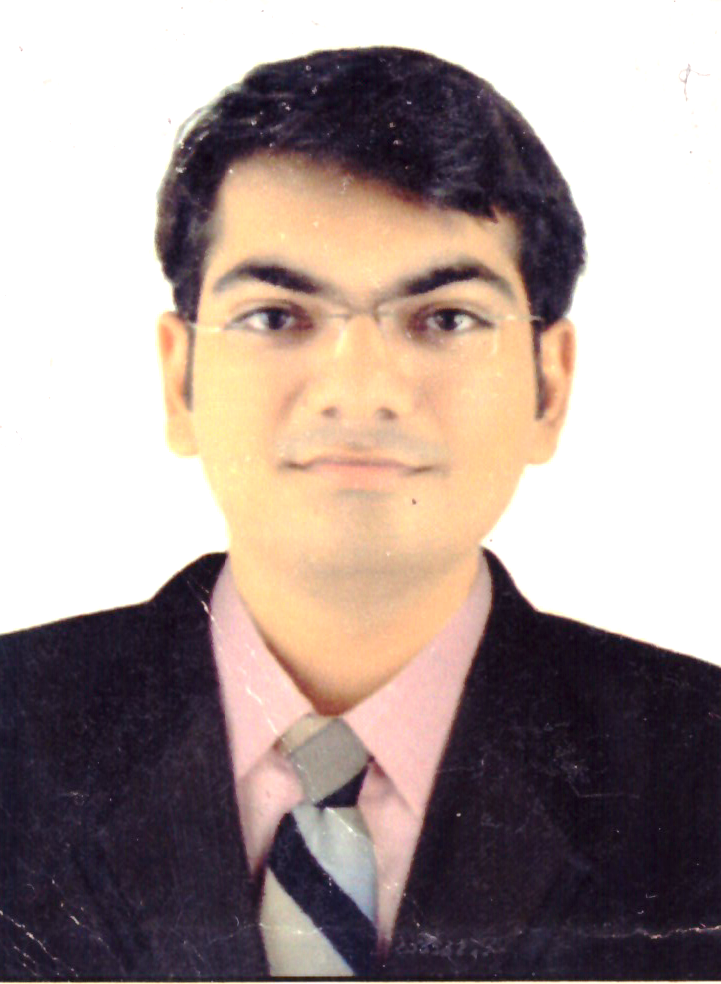
\includegraphics[scale=0.9, valign=c]{cv.png}
    \end{tabular}

%----------------------------------------------------------------------------------------
%	EXPERIENCE
%----------------------------------------------------------------------------------------

\section{Work Experience}
\begin{tabular}{cp{11.5cm}}	
	\textsc{November} 2021 --  & \textbf{Research Assistant}, School of Data Analysis and Artificial Intelligence \\
	\textsc{Present}& \textbf{Faculty of Computer Science, Higher School of Economics}, Moscow  \\
	\\
	\textsc{November} 2021 --  & \textbf{Internatioanl Sales Advisor (Coordinator)} , Export Department, \\
	\textsc{April} 2021 & \textbf{Varmora Granito Pvt. Ltd. (Varmora Group)}, India\\
	\\
	\textsc{August} 2019 --  & \textbf{Assistant Professor} , Information \& Communication Technology, \\
	\textsc{May} 2021 & \textbf{Marwadi Education Foundation (Marwadi University)}, India 
\end{tabular}

%----------------------------------------------------------------------------------------
%	EDUCATION
%----------------------------------------------------------------------------------------

\section{Education}
\begin{tabular}{cp{15.5cm}}	
\textsc{November} 2021 --  & {Ph.D.} {(2\textsuperscript{nd} Year)} , Faculty of Computer Science, \\
\textsc{Present}& \textbf{Higher School of Economics}, Moscow | \scriptsize Advisor: Prof. Attila K. \textsc{Farkas} \\
& \scriptsize Thesis: ``Exact p-value calculation for high resolution Tandem Mass Spectrometry data.'' \\
\\
\textsc{July} 2017 --  & Master of Technology , Control and Automation, \\
\textsc{April} 2019& \textbf{Vellore Institute of Technology}, India | \scriptsize Advisor: Prof. Monica M. \textsc{Subashini} \\
& \scriptsize  Thesis: ``Automatic Bird Deterrent and Repellent System for Airfield.'' | \normalsize \textsc{Cgpa}: 8.39/10.0  \\
\\
\textsc{September} 2018 --  & Research Exchange Internship , Automation and Mechatronics, \\
\textsc{June} 2019& \textbf{Saint Petersburg Electrotechnical University "LETI"}, Russia \\
& \scriptsize Advisor: Prof.Anastasia  D. \textsc{Skakun} \qquad \qquad \qquad  \qquad \qquad \qquad \qquad \quad \: \ | \normalsize \textsc{Cgpa}: 4.8/5.0  \\
\\
\textsc{July} 2012 --  & Bachelor of Engineering , Instrumentation and Control, \\
\textsc{June} 2016& \textbf{Gujarat Technological University}, India \qquad \qquad \ | \normalsize \textsc{Cgpa}: 7.28/10.0\\
\end{tabular}

%----------------------------------------------------------------------------------------
%	Achievments
%----------------------------------------------------------------------------------------

\section{Achievments \& Scholarships }
\begin{tabular}{rp{8cm}r}
	\textsc{December} 2022 | & Bootcamp Hackathon | Machine Learning From Scratch 2022 \footnotesize(2\textsuperscript{nd} Runner Up)\normalsize&\href{https://www.hse.ru/ma/mds/hackathon/}{\hfill | \footnotesize Certificate}\\
	
	\textsc{April} 2019,2021,2022 | & Open Door: Russian Scholarship Project \scriptsize(3-times Winner)&\href{https://www.od.globaluni.ru/en/}{\hfill | \footnotesize Certificate}\\
	\vspace*{20pt}	
	\textsc{May} 2019 | & Study Abroad Scholarship: VIT University \scriptsize(Travel grant)
\end{tabular}

% ----------------------------------------------------------------------------------------
% 	PUBLICATION
% ----------------------------------------------------------------------------------------

\section{Publications}
\begin{tabular}{r|p{12cm}}
    \textsc{Article} & Kertesz-Farkas A., Adoquaye Acquaye F. L. N., Bhimani K., Eng J. K., Fondrie W. E., Hoopmann M. R., Lin A., MacCoss M. J., and Noble W. S. (2022). "The Crux toolkit for analysis of bottom-up tandem mass spectrometry proteomics data." Cold Spring Harbor Laboratory. \href{https://pubs.acs.org/doi/full/10.1021/acs.jproteome.2c00615}{\qquad \qquad \qquad \qquad \qquad \qquad \qquad\;\;| \footnotesize{Paper}}\\ \multicolumn{2}{c}{}\\
    & S. Manna, S. Ghildiyal and K. Bhimani, "Face Recognition from Video using Deep Learning," 2020 5th International Conference on Communication and Electronics Systems (ICCES), 2020, pp. 1101-1106,\href{https://ieeexplore.ieee.org/abstract/document/9137927}{ \qquad \qquad \qquad \qquad \qquad \;\;\;| \footnotesize{Paper}}\\ \multicolumn{2}{c}{}\\
    & G. R. V. Ponce, K. Bhimani, J. A. Prakosa and M. A. B. Alvarez, "Pattern Recognition Through Digital Image Processing for Unmanned Aerial Vehicles," 2019 IEEE XXVI International Conference on Electronics, Electrical Engineering and Computing (INTERCON), 2019, pp. 1-4,\href{https://ieeexplore.ieee.org/abstract/document/8853558}{\qquad \qquad \qquad \qquad \qquad \qquad \qquad \;\;\; | \footnotesize{Paper}}\\ \multicolumn{2}{c}{}\\
    & S. Ghildiyal, K. Bhimani, G. Mani, M. Subashini and A. Stotckaia, "Control of Wheeled Mobile Robot Using Centroid Algorithm," 2019 Innovations in Power and Advanced Computing Technologies, 2019, pp. 1-4,\href{https://ieeexplore.ieee.org/abstract/document/8959523}{\hfill | \footnotesize{Paper}}\\ \multicolumn{2}{c}{}\\
    & S. Ghildiyal, K. Bhimani and Manimozhi, "Design To Convert a Wired PLC into Wireless PLC," 6 Issue. 2321-9653.,\href{https://www.ijraset.com/fileserve.php?FID=13054}{\hfill | \footnotesize{Paper}}\\ \multicolumn{2}{c}{}\\
    
\end{tabular}

\section{Training}
\begin{tabular}{rp{10cm}}
	\vspace*{5.33pt}
    \textsc{January} 2023 & Winter School on Analytics \& Data Science \footnotesize(by HSE University)\normalsize \\
	\vspace*{5.33pt}
    \textsc{April-July} 2022 & GoogleCloudReady Facilitator Program \footnotesize(by Google cloud \& Qwiklabs)\normalsize\\

    \textsc{February-March} 2019 & Mechatronics and Robotics \footnotesize(Winter School at LETI University)\normalsize

    \end{tabular}

\section{Projects}
\begin{tabular}{p{14.5 cm}}
\begin{center}\vspace*{-7.8pt}

\begin{enumerate}[wide, itemsep=6.66pt, leftmargin=*]
%    \item \textsc{Style transfer telegram bot} \href{https://github.com/addicted-by/nst_bot}{\hfill | \footnotesize Link}\\[3.33pt] Asynchronized telegram with simple database to neural photo stylization\\[3.33pt] \textsc{Stack}: \py{aiogram} \py{sqlite} \py{torch} \py{torchvision} \mytcbox{GAN}
    \item \textsc{Crux toolkit for mass spectrometry data analysis} \href{https://github.com/MrBhimani/crux-toolkit}{\hfill | \footnotesize Link}\\[2.5pt] Open Source project to provide group of algorithms and search tools for MS-MS Analysis \\[3.33 pt] \textsc{Stack}: \py{Python} \; \html{\textsc{Bootstrap}} \; \mytcbox{\textsc{C / C++}} \; \mytcbox{Shell Script} \; \mytcbox{\textsc{Proteomics Toolkit \& Algorithms} }
    \item \textsc{Social media analysis for virus vulnerability detection} \href{https://github.com/MrBhimani/Social_Media_Analysis}{\hfill | \footnotesize Link}\\[3.33 pt] To provide meaningful insights about Social media analysis by crafting policy \& regulations\\[7.33pt] \textsc{Stack}: \py{TwitterBotAPI} \; \py{Colab} \; \py{\textsc{Exploratory \& Sentiment Data Analysis}} \; \mytcbox{\textsc{Time Series}  }
    \item \textsc{Bird control analysis \& repellent system for airports} \href{https://docs.google.com/document/d/1Vcn2ZzZxH46hQ6s7orPIyeZQj4_RFs2fnz81Rq-qs2I/edit}{\hfill | \footnotesize Link}\\[3.33pt] Technological solution for removing airborne animals and avoid plane bird strikes \\[3.33pt] \textsc{Stack}: \py{Python}  \mytcbox{\textsc{Image Processing}}  \mytcbox{\textsc{Computer Vision}} \mytcbox{\textsc{Arduino}} \mytcbox{\textsc{Bird Repellent \& Deterrent}}
\end{enumerate} \vspace*{-10pt}
\end{center}
\end{tabular}
    

% CROC case laboratory
% High Quality Award
% ISS HACK
%----------------------------------------------------------------------------------------
%	LANGUAGES
%----------------------------------------------------------------------------------------

\section{Languages}

\begin{tabular}{rl}
\textsc{English:} & Fluent \qquad \qquad \qquad   \textsc{Gujarati:} \enspace Mother tongue \qquad \qquad \textsc{Sanskrit:} \enspace Intermediate \\

\textsc{Hindi:} & Professional \qquad \enspace \enspace \enspace  \  \textsc{Russian:} \enspace Basic \qquad \qquad \qquad \enspace \enspace \enspace \enspace \: \   \textsc{German:} \enspace Basic\\

\end{tabular}

\section{Relevant Courses \& Specialization}
\begin{tabular}{rp{11cm}r}
	\textsc{December 2022} &  Mathematics for Machine Learning: Specialization \footnotesize(3 Courses)\normalsize\href{https://coursera.org/verify/specialization/TXDLZSR9792P}{\hfill | \footnotesize Certificate}\\
	\textsc{December 2022} & SQL for Data Science \footnotesize(by University of California, Davis)\normalsize\href{https://coursera.org/verify/UE3N5M4WRRDK}{\hfill | \footnotesize Certificate} \\
	\textsc{August 2022} & Python: From Scratch to Data Visualization \footnotesize(by HSE University)\normalsize\href{https://drive.google.com/file/d/1YRf4fjrd9PRfQaVNCkcWe9OTWG-HjbqU/view?usp=share_link}{\hfill | \footnotesize Certificate}\\
    \textsc{October 2020} & AI in Healthcare: Specialization \footnotesize(5 Courses)\normalsize\href{https://coursera.org/verify/specialization/QM3JUXZS9FS3}{\hfill | \footnotesize Certificate}\\
    \textsc{August 2020} & Python for Everybody Specialization \footnotesize(by University of Michigan)\normalsize\href{https://coursera.org/verify/RVTZSMMVGH3K}{\hfill | \footnotesize Certificate}\\
    \textsc{May 2020} & Introduction to TensorFlow for AI, ML, and DL \footnotesize\normalsize\href{https://coursera.org/verify/42WLFE8NLMRF}{\hfill | \footnotesize Certificate}\\
    \textsc{April 2020} &  Machine Learning {by Stanford Online} \footnotesize(by Andrew NG)\normalsize\href{https://coursera.org/verify/9QAAQEEFQYGG}{\hfill | \footnotesize Certificate}\\
    
    
\end{tabular}


%----------------------------------------------------------------------------------------
%	INTERESTS AND ACTIVITIES
%----------------------------------------------------------------------------------------

\section{Interests and Activities}

Programming \: |\: Reading \: |\: Cycling \: |\: Meditation \: |\: Hosting Activities \: |\:  Drama artist. \\

%----------------------------------------------------------------------------------------

\newpage


\end{document}
